\documentclass[12pt]{article}
%Also I made it 12pt

\usepackage[fontset=macnew]{ctex}
\usepackage{physics}
\usepackage{tikz}
\usetikzlibrary{3d,calc,patterns}
% \usepackage{tkz-euclide}
\usepackage{amsmath}
\usepackage{upgreek}
\usepackage{amsthm}
\usepackage{amsfonts}
\usepackage{mathrsfs}
% \usepackage{subfigure}
\usepackage{subcaption}
%to add an affiliation line to the the title formatting
\usepackage{authblk}

%Fonts
% \usepackage[no-math]{fontspec} %This allows you to enter (via an IPA kayboard) IPA fonts and other symbols directly into LaTeX. Requires a particular setyp, see below.
\usepackage{libertine} %A font that actually contains many IPA symbols. This is the font you see in the preview to the right.

%to use these fonts, be sure that your typesetting engine is set to "XeLaTeX." In Overleaf, go to the Menu link on the top left (by the Overleaf icon), and under Settings be sure that the Compiler is set to "XeLaTeX." If you accessed this document via the Overleaf Pomona Linguistics template, all of this was already done for you.

%The Pomona Linguistics Paper Template in Overleaf is already set up for this, but you may run into this problem if you start building your own documents.


%%%%%%%%%%%%%%%%%%%%%%%%%%%%%%%%%%%%%%%%%%%%%%%%%%%
%packages for this style of handout-formatting of (sub)section headers 
\usepackage[explicit]{titlesec}
\usepackage{xcolor}

\definecolor{light-gray}{gray}{0.7}
\definecolor{lighter-gray}{gray}{0.85}

\titleformat{\section}
{\normalfont\Large\bfseries}{}{0em}{\colorbox{black}{\parbox{\dimexpr\textwidth-2\fboxsep\relax}{\textcolor{white}{\thesection\quad#1}}}}

\titleformat{\subsection}
{\normalfont\large\bfseries\scshape}{}{0em}{\colorbox{light-gray}{\parbox{\dimexpr\textwidth-2\fboxsep\relax}{\textcolor{black}{\thesubsection\quad#1}}}}

\titleformat{\subsubsection}
{\normalfont\bfseries}{}{0em}{\colorbox{lighter-gray}{\parbox{\dimexpr\textwidth-2\fboxsep\relax}{\textcolor{black}{\thesubsubsection\quad#1}}}}
%%%%%%%%%%%%%%%%%%%%%%%%%%%%%%%%%%%%%%%%%%%%%%%%%%%

%%% This file is the preamble for the Pomona Linguistics LaTeX Paper Template, which is also used for the Quick Reference Guide. If you are brand new to writing with LaTeX, we suggest NOT messing with it, and just writing your paper using the Paper Template. If you are getting more comfortable in LaTeX and want to add packages and commands, this is where you do it (when using this template).

%For stacking text, used here in autosegmental diagrams
\usepackage{stackengine}

%To combine rows in tables
\usepackage{multirow}

%geometry helps manage margins, among other things.
\usepackage[margin=1in]{geometry}

%Gives some extra formatting options, e.g. underlining/strikeout
\usepackage{ulem}

%For putting links into papers, also helps make cross-references in the paper smart references
\usepackage[colorlinks = true,
            linkcolor = blue,
            urlcolor  = blue,
            citecolor = blue,
            anchorcolor = blue]{hyperref} %smarter cross-references, these options turn links blue

%Use package/command below to create a double-spaced document, if you want one. Uncomment BOTH the package and the command (\doublespacing) to create a doublespaced document, or leave them as is to have a single-spaced document.
%\usepackage{setspace}
%\doublespacing 

%paragraph formatting
\usepackage[parfill]{parskip}
\setlength{\parskip}{5pt} %plus 1 minus 1}
\setlength{\parindent}{30pt}
\usepackage{titlesec}

%use for special OT tableaux symbols like bomb and sad face. must be loaded early on because it doesn't play well with some other packages
\usepackage{fourier-orns}

%Basic math symbols 
\usepackage{pifont}
\usepackage{amssymb}

%%%Gives shortcuts for glossing. The use of this package is NOT explained in the Quick Reference Guide, but the documentation is on CTAN for those that are interested. MJKD finds it handy for glossing. (https://ctan.org/pkg/leipzig?lang=en)
\usepackage{leipzig}

%Tables
\usepackage{caption} %For table captions
\usepackage{booktabs} %helps format tables

%For citations and bibliography - as of 9.1.2019 we don't explain citations in this Quick Reference Guide, but Pedro Martin's tutorial does (see links in the Guide).
\usepackage{natbib}

%For OT-style tableaux
\usepackage{ot-tableau}

%highlights text with \hl{text}
\usepackage{color, soul}

%Drawing Syntax Trees
\usepackage[linguistics]{forest}

%This specifies some formatting for the forest trees to make them nicer to look at
\forestset{
  nice nodes/.style={
    for tree={
      inner sep=0pt,
      fit=band,
    },
  },
  default preamble=nice nodes,
}

%% For numbered and glossed examples %%
\usepackage{gb4e}



%Changes the \maketitle command to be smaller and take up less space on a page. 
\makeatletter         
\def\@maketitle{   % custom maketitle 
\noindent {\Large \bfseries \color{black} \@title}  \\ \hrule \noindent \@author \\ \@date  
}

%The code below will draw a circle around a piece of text. This is very useful for drawing attention to a word in a data example. use the command \circled{text} where the argument (`text' here) is what you want to be circled. This is illustrated in the Quick Reference Guide and the Paper Template.

\usepackage{tikz}

\newcommand{\circled}[1]{\begin{tikzpicture}[baseline=(word.base)]
\node[draw, rounded corners, text height=8pt, text depth=2pt, inner sep=2pt, outer sep=0pt, use as bounding box] (word) {#1};
\end{tikzpicture}
}


%%%%%%%%%%%%%%%%%%%%%%%%%%%%%%%%%%%%%%%%%%%%%%%%%%%%%%%%%%%%
%%%%%%%%%%%%%%%%%%%%%%%%%%%%%%%%%%%%%%%%%%%%%%%%%%%%%%%%%%%%

% Useful Ling Shortcuts

\RequirePackage{leipzig}
%\RequirePackage{mathtools} % for \mathrlap

% % % Shortcuts  (borrowed from JZ, I'm still unsure exactly what xspace requires)
\RequirePackage{xspace}
\xspaceaddexceptions{]\}}

%This makes the \emptyset command be a nicer one
\let\oldemptyset\emptyset
\let\emptyset\varnothing
\newcommand{\nothing}{$\emptyset$}

%Not all of these are explained in the Quick Reference Guide, but they are here bc they are relevant to some of our students.
\newcommand{\1}{\rlap{$'$}\xspace}
\newcommand{\0}{\rlap{\textsuperscript{$ˆ{\circ}$}}\xspace}
\newcommand{\Lb}[1]{$\text{[}_{\text{#1}}$ } %A more convenient left bracket
\newcommand{\Rb}[1]{$\text{]}_{\text{#1}}$ } %A more convenient left bracket
\newcommand{\gap}{\underline{\hspace{1.2em}}}
\newcommand{\vP}{\emph{v}P}
\newcommand{\lilv}{\emph{v}}
\newcommand{\Abar}{A$'$-} %A more convenient A-bar notation
\newcommand{\ph}{$\varphi$\xspace} %A more convenient phi
\newcommand{\pro}{\emph{pro}\xspace}
\newcommand{\subs}[1]{\textsubscript{#1}} %A more convenient subscript
%\newcommand{\hd}{$^{\circ}$\xspace} %Symbol for printing head / degree symbol
\newcommand{\spells}{$\Longleftrightarrow$} %spellout arrow for morph spellout rules
% \newcommand{\tr}[1]{\textit{t}\textsubscript{\textit{#1}}} %easy traces with subscript
\newcommand{\supers}[1]{\textsuperscript{#1}}

% Abbreviations for glossing, based on Leipzig
\newleipzig{hab}{hab}{habitual}
\newleipzig{rem}{rem}{remote}
\newleipzig{sm}{sm}{subject marker}
\newleipzig{t}{t}{tense}
\newleipzig{aa}{aa}{anti-agreement}
\newleipzig{pron}{pron}{pronoun}
\newleipzig{rec}{rec}{recent}
\newleipzig{om}{om}{object marker}
%\newleipzig{ipfv}{ipfv}{imperfective}
\newleipzig{asp}{asp}{aspect}
\newleipzig{lk}{lk}{linker}
\newleipzig{pcl}{pcl}{particle}
\newleipzig{stat}{stat}{stative}
\newleipzig{ints}{ints}{intensive}
\newleipzig{ascl}{ascl}{assertive subject clitic}
\newleipzig{nascl}{nascl}{non-assertive subject clitic}
\newleipzig{ta}{ta}{tense and/or aspect}
\newleipzig{assoc}{assoc}{associative marker}
\newleipzig{hon}{hon}{honorific}
%\newleipzig{whprt}{wh}{\wh particle}
\newleipzig{sa}{sa}{subject agreement}
\newleipzig{conj}{conj}{conjunction}
%\newleipzig{loc}{loc}{locative}
\newleipzig{expl}{expl}{expletive}
\newleipzig{rcm}{rcm}{reciprocal marker}
\newleipzig{pers}{pers}{persistive}
%\newleipzig{}{}{} %this is just to copy for when I want to add more

%%%%%%%%%%%%%%%%%%%%%%%%%%%%%%%%%%%%%%%%%%%%%%%%%%%%%%%%%%%%
%%%%%%%%%%%%%%%%%%%%%%%%%%%%%%%%%%%%%%%%%%%%%%%%%%%%%%%%%%%%

%A couple of packages that seemed to prefer being called toward the end of the preamble

%This package provides macros for typesetting SPE-style phonological rules.
\usepackage{phonrule}

%For using Greek letters outside of math mode.
\usepackage{textgreek}


%Random, lets us use the XeLaTeX logo. Not important to the template at all.
\usepackage{metalogo}


%%%%%%%%%%%%
%% This is the end of the PREAMBLE
%%%%%%%%%%%

%MJKD note to future self - this preamble is just the section headers + PomLing formatting, but an ordering paradox between the two files made me combine them and re-order fontspec. *shrug* In future if it needs an update, just take the PomLing formatting file and add in the section headers for handouts.

\newcommand{\rmd}{\mathrm{d}}
\newcommand{\deriv}[2]{\frac{\rmd #1}{\rmd #2}}
\newcommand{\pderiv}[2]{\frac{\partial #1}{\partial #2}}
\newcommand{\dpderiv}[2]{\dfrac{\partial #1}{\partial #2}}
\newcommand{\dderiv}[2]{\dfrac{\rmd #1}{\rmd #2}}

\title{电磁场与电磁波}
\author{\href{mailto:lai-wei@whu.edu.cn}{Lai Wei}}
\date{\today}

\begin{document}

\maketitle

\section{位移电流 \quad 全电流安培环路定理}

\subsection{位移电流}

麦克斯韦认为,可以把电位移通量对时间的变化率看做是一种电流,称作是位移电流,用\(I_D\)表示;把电位移矢量对时间的变化率称为位移电流密度,用\(j_D\)表示。于是定义

位移电流密度
\begin{equation}
    \overrightarrow{j}_D = \pderiv{\overrightarrow{D}}{t}
\end{equation}

位移电流
\begin{equation}
I_{\mathrm{d}}=\deriv{\varPsi}{t} = \int_S \pderiv{\overrightarrow{D}}{t} \cdot \rmd \overrightarrow{S}
\end{equation}

\subsection{全电流安培环路定理}

麦克斯韦认为:在非恒定电流的电路中,存在着两种电流,一种是电荷的定向移动形成的传导电流,另一种是电位移通量的变化引起的位移电流,两种电流的总和称为全电流,并用\(I_S\)表示,即
\begin{equation}
    I_S = I_C + I_D = \int_S \overrightarrow{j}_C \cdot \rmd \overrightarrow{S} + \int \pderiv{\overrightarrow{D}}{t} \cdot \rmd S
\end{equation}
在非恒定电流情况下,电路中的传导电流虽然不连续,但是全电流总是连续的。

在考虑了全电流概念以后,麦克斯韦将磁场的安培环路定理推广为
\begin{equation}
\oint_L \overrightarrow{H} \cdot \mathrm{~d} \overrightarrow{L}=I_{\mathrm{S}}=I_{\mathrm{C}}+I_{\mathrm{D}}=\int_S \overrightarrow{j}_{\mathrm{C}} \cdot \mathrm{~d} \overrightarrow{S}+\int_S \frac{\partial \overrightarrow{D}}{\partial t} \cdot \mathrm{~d} \overrightarrow{S}
\label{15-4}
\end{equation}
式\ref{15-4}称为全电流安培环路定理。该定理表明,磁场强度对于任意闭合回路的环流等于该闭合回路所包围的(也就是穿过以该回路为周界的任意曲面的)全电流。式\ref{15-4}中的\(\overrightarrow{H}\)是空间所有电流(闭合回路内外的所有传导电流和位移电流)所共同产生的。该定理的意义在于指出了传导电流和位移电流都会激发涡施磁场,并且以完全相同的方式激发磁场。由于位移电流本质上就是变化的电场,因此麦克斯书关于位移电流假设的本质是认为变化的电场也能激发涡旋磁场。

应当注意:传导电流和位移电流尽管在激发涡旋磁场的规律上是相同的,但它们是两种完全不同的电流。

\section{麦克斯韦方程组}

\subsection{麦克斯韦方程组的积分形式}

在19世纪中期确立了电荷、电流和电场、磁场之间的普遍关系后,麦克斯韦建立了统一的电磁场理论。他指出,除静止电荷激发无旋电场外,变化的磁场还将激发涡旋电场;同时,变化的电场和传导电流一样激发涡旋磁场。这就是说,变化的电场和变化的磁场不是彼此孤立的,它们相互联系、相互激发组成一个统一的电磁场。下面我们根据麦克斯韦的这些基本概念,首先介绍由他总结出来的麦克斯韦电磁场方程组(Maxwell equations)的积分形式。

麦克斯韦认为,在一般情况下,空间的总电场强度\(\overrightarrow{E}\)是静电场\(\overrightarrow{E}_{\text{静}}\)和感生电场\(\overrightarrow{E}_{\text{感}}\)的矢量和,即
\begin{equation}
    \overrightarrow{E} = \overrightarrow{E}_{\text{静}} + \overrightarrow{E}_{\text{感}}
\end{equation}
同理,总电位矢量\(\overrightarrow{D}\)为
\begin{equation}
    \overrightarrow{D} = \overrightarrow{D}_{\text{静}} + \overrightarrow{D}_{\text{感}}
\end{equation}

由于静电场是有源、无旋的,感生电场是无源、有旋的,所以总电流强度\(\overrightarrow{E}\)对任意闭合回路\(L\)的环流为
\begin{equation*}
\begin{aligned}
\oint_L \overrightarrow{E} \cdot \mathrm{~d} \overrightarrow{L} & =\oint_L\left(\overrightarrow{E}_{\text {静}}+\overrightarrow{E}_{\text {感}}\right) \cdot \mathrm{d} \overrightarrow{L} \\
& =\oint_L \overrightarrow{E}_{\text {静}} \cdot \mathrm{d} \overrightarrow{L}+\oint_L \overrightarrow{E}_{\text {感}} \cdot \mathrm{d} \overrightarrow{L}=0+\left(-\frac{\mathrm{d} \Phi}{\mathrm{~d} t}\right)=-\int_S \frac{\partial \overrightarrow{B}}{\partial t} \cdot \mathrm{~d} \overrightarrow{S}
\end{aligned}
\end{equation*}
即
\begin{equation}
\oint_L \overrightarrow{E} \cdot \mathrm{~d} \overrightarrow{L}=-\int_S \frac{\partial \overrightarrow{B}}{\partial t} \cdot \mathrm{~d} \overrightarrow{S}
\label{15-7}
\end{equation}
式中\(S\)是以\(L\)为周界的任一曲面。总电位移矢量\(\overrightarrow{D}\)对任意闭合曲面的通量为
\begin{equation*}
\oint_S \overrightarrow{D} \cdot \mathrm{~d} \overrightarrow{S}=\oint_S \overrightarrow{D}_{\text {静}} \cdot \mathrm{d} \overrightarrow{S}+\oint_S \overrightarrow{D}_{\text {感 }} \cdot \mathrm{d} \overrightarrow{S}=\sum q+0=\int_V \rho \mathrm{~d} V
\end{equation*}
即
\begin{equation}
\oint_S \overrightarrow{D} \cdot \mathrm{~d} \overrightarrow{S}=\int_V \rho \mathrm{~d} V
\label{15-8}
\end{equation}
式中的积分体积\(V\)是闭合曲面\(S\)所围的体积\(\rho\)是自由电荷密度。

对于磁场,麦克斯韦同样认为,在一般情况下,空间的磁场是由恒定电流和位移电流共同产生的,磁场的环路定理应服从全电流安培环路定理,即
\begin{equation}
\oint_L \overrightarrow{H} \cdot \mathrm{~d} \overrightarrow{L}=\int_S \overrightarrow{j}_{\mathrm{C}} \cdot \mathrm{~d} \overrightarrow{S}+\int_S \frac{\partial \overrightarrow{D}}{\partial t} \cdot \mathrm{~d} \overrightarrow{S}
\label{15-9}
\end{equation}
由于恒定电流和位移电流都是无源的涡旋场,所以,磁场的高斯定理的形式不变,即
\begin{equation}
\oint_S \overrightarrow{B} \cdot \mathrm{~d} \overrightarrow{S}=0
\label{15-10}
\end{equation}

由方程式\ref{15-7}、方程式\ref{15-8}、方程式\ref{15-9}、方程式\ref{15-10}所构成的方程组
\begin{equation}
\displaystyle
\left\{\begin{array}{l}
\oint_S \overrightarrow{D} \cdot \mathrm{~d} \overrightarrow{S}=\int_V \rho \mathrm{~d} V \\
\oint_L \overrightarrow{E} \cdot \mathrm{~d} \overrightarrow{L}=-\int_S \frac{\partial \overrightarrow{B}}{\partial t} \cdot \mathrm{~d} \overrightarrow{S} \\
\oint_S \overrightarrow{B} \cdot \mathrm{~d} \overrightarrow{S}=0 \\
\oint_L \overrightarrow{H} \cdot \mathrm{~d} \overrightarrow{L}=\int_S \overrightarrow{j}_{\mathrm{C}} \cdot \mathrm{~d} \overrightarrow{S}+\int_S \frac{\partial \overrightarrow{D}}{\partial t} \cdot \mathrm{~d} \overrightarrow{S}
\end{array}\right.
\end{equation}
就是著名的麦克斯韦方程组的积分形式。

\subsection{麦克斯韦方程组的微分形式}

\section{电磁波}

\subsection{LC电磁振荡}

一个不计电阻的LC电路,就可以实现电磁振荡,故也称LC振荡电路。
\begin{figure}[!h]
    \centering
    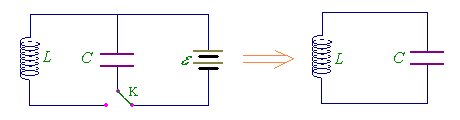
\includegraphics[width = .8\textwidth]{graphics/LC振荡电路.png}
\end{figure}

可以证明,LC振荡电路的振荡频率为
\begin{equation}
    \nu = \frac{1}{2 \uppi \sqrt{LC}}
\end{equation}

\subsection{电磁波的产生和传播}

我们将电矩随时间作迅速周期性变化的电偶极子称为振荡电偶极子。最简单的振荡电偶极子模型是电矩随时间按余弦或正弦规律进行变化,即
\begin{equation*}
    \overrightarrow{p} = \overrightarrow{p}_0 \cos \omega t
\end{equation*}

若以振荡电偶极子的中心位坐标原点,以振子轴线为极轴的球坐标来描述电磁场,通过求解麦克斯韦方程组可以得到,在\(r >> \lambda\)的波长总任意一点P处的电场强度\(\overrightarrow{E}\)和磁场强度\(\overrightarrow{H}\)的数值分别为
\begin{equation}
    E(r, t)=\frac{p_0 \omega^2 \sin \theta}{4 \pi \varepsilon u^2 r} \cos \omega\left(t-\frac{r}{u}\right)
\end{equation}
\begin{equation}
    H(r, t)=\frac{p_0 \omega^2 \sin \theta}{4 \pi u r} \cos \omega\left(t-\frac{r}{u}\right)
\end{equation}
式中\(\omega\)为振荡电偶极子的角频率,\(p_0\)为振荡电偶极子电矩的振幅,\(r\)为振荡电偶极子中心到P点的位矢\(\overrightarrow{r}\)的大小,\(\theta\)为位矢\(\overrightarrow{r}\)与极轴的夹角,\(u\)为电磁波的传播速度。\(\varepsilon = \varepsilon_0 \varepsilon_r\),\(\mu = \mu_0 \mu_r\)

可以证明,电磁波的传播速度为
\begin{equation}
    u = \frac{1}{\sqrt{\mu \varepsilon}}
\end{equation}

此外,在波长中任一点P处,\(\overrightarrow{E}\)和\(\overrightarrow{H}\)的方向与波的传播方向垂直,并成右手螺旋关系。

\end{document}